\nobreak
Next we consider series with both positive and negative terms, but in
a regular pattern: the signs alternate, as in the {\dfont alternating
  harmonic series\index{alternating harmonic series}%
\index{harmonic series!alternating}%
\index{series!alternating harmonic}\/} for example:
\begin{align*}
  \sum_{n=1}^\infty {(-1)^{n+1}\over n}
  &={1\over1}+{-1\over2}+{1\over3}+{-1\over4}+\cdots \\
  &= {1\over1}-{1\over2}+{1\over3}-{1\over4}+\cdots.
\end{align*}
In this series the sizes of the terms decrease, that is, 
$\ds |a_n|$ forms a decreasing sequence, but this is not required in an
alternating series. As with positive term series, however, when the
terms do have decreasing sizes it is easier to analyze the series,
much easier, in fact, than positive term series. Consider pictorially
what is going on in the alternating harmonic series, shown in
Figure~\xrefn{fig:alternating-harmonic-series}. Because the sizes of
the terms $\ds a_n$ are decreasing, the partial sums $\ds s_1$, $\ds s_3$, $\ds s_5$,
and so on, form a decreasing sequence that is bounded below by
$\ds s_2$, so this sequence must converge.
Likewise, the partial sums $\ds s_2$, $\ds s_4$, $\ds s_6$,
and so on, form an increasing sequence that is bounded above by
$\ds s_1$, so this sequence also converges. Since all the even numbered
partial sums are less than all the odd numbered ones, and since the
``jumps'' (that is, the $\ds a_i$ terms) are getting smaller and smaller,
the two sequences must converge to the same value, meaning the entire
sequence of partial sums $\ds s_1,s_2,s_3,\ldots$ converges as well.

\begin{fullwidth}
\begin{figure}[!h]
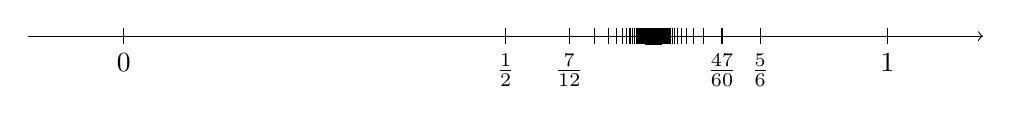
\begin{tikzpicture}[line width=0.4pt]
\draw [->] (0,0) -- (\textwidth,0);
\draw (0.1\textwidth,-0.1) -- (0.1\textwidth,0.1);
\draw (0.9\textwidth,-0.1) -- (0.9\textwidth,0.1);
\node[anchor=north] (zero) at (0.1\textwidth,-0.1) {$0$};
\node[anchor=north] (one) at (0.9\textwidth,-0.1) {$1$};
\draw (0.5\textwidth,-0.1) -- (0.5\textwidth,0.1);
\node[anchor=north] (half) at (0.5\textwidth,-0.1) {$\frac{1}{2}$};
\draw (0.766666666666667\textwidth,-0.1) -- (0.766666666666667\textwidth,0.1);
\node[anchor=north] (a3) at (0.766666666666667\textwidth,-0.1) {$\frac{5}{6}$};
\draw (0.566666666666667\textwidth,-0.1) -- (0.566666666666667\textwidth,0.1);
\node[anchor=north] (a4) at (0.566666666666667\textwidth,-0.1) {$\frac{7}{12}$};
\draw (0.726666666666667\textwidth,-0.1) -- (0.726666666666667\textwidth,0.1);
\node[anchor=north] (a5) at (0.726666666666667\textwidth,-0.1) {$\frac{47}{60}$};
\draw (0.593333333333333\textwidth,-0.1) -- (0.593333333333333\textwidth,0.1);
\draw (0.707619047619048\textwidth,-0.1) -- (0.707619047619048\textwidth,0.1);
\draw (0.607619047619048\textwidth,-0.1) -- (0.607619047619048\textwidth,0.1);
\draw (0.696507936507937\textwidth,-0.1) -- (0.696507936507937\textwidth,0.1);
\draw (0.616507936507937\textwidth,-0.1) -- (0.616507936507937\textwidth,0.1);
\draw (0.689235209235209\textwidth,-0.1) -- (0.689235209235209\textwidth,0.1);
\draw (0.622568542568543\textwidth,-0.1) -- (0.622568542568543\textwidth,0.1);
\draw (0.684107004107004\textwidth,-0.1) -- (0.684107004107004\textwidth,0.1);
\draw (0.626964146964147\textwidth,-0.1) -- (0.626964146964147\textwidth,0.1);
\draw (0.680297480297480\textwidth,-0.1) -- (0.680297480297480\textwidth,0.1);
\draw (0.630297480297480\textwidth,-0.1) -- (0.630297480297480\textwidth,0.1);
\draw (0.677356303826892\textwidth,-0.1) -- (0.677356303826892\textwidth,0.1);
\draw (0.632911859382448\textwidth,-0.1) -- (0.632911859382448\textwidth,0.1);
\draw (0.675017122540342\textwidth,-0.1) -- (0.675017122540342\textwidth,0.1);
\draw (0.635017122540342\textwidth,-0.1) -- (0.635017122540342\textwidth,0.1);
\draw (0.673112360635580\textwidth,-0.1) -- (0.673112360635580\textwidth,0.1);
\draw (0.636748724271944\textwidth,-0.1) -- (0.636748724271944\textwidth,0.1);
\draw (0.671531332967596\textwidth,-0.1) -- (0.671531332967596\textwidth,0.1);
\draw (0.638197999634263\textwidth,-0.1) -- (0.638197999634263\textwidth,0.1);
\draw (0.670197999634263\textwidth,-0.1) -- (0.670197999634263\textwidth,0.1);
\draw (0.639428768865032\textwidth,-0.1) -- (0.639428768865032\textwidth,0.1);
\draw (0.669058398494662\textwidth,-0.1) -- (0.669058398494662\textwidth,0.1);
\draw (0.640486969923233\textwidth,-0.1) -- (0.640486969923233\textwidth,0.1);
\draw (0.668073176819785\textwidth,-0.1) -- (0.668073176819785\textwidth,0.1);
\draw (0.641406510153118\textwidth,-0.1) -- (0.641406510153118\textwidth,0.1);
\draw (0.667212961766022\textwidth,-0.1) -- (0.667212961766022\textwidth,0.1);
\draw (0.642212961766021\textwidth,-0.1) -- (0.642212961766021\textwidth,0.1);
\draw (0.666455386008446\textwidth,-0.1) -- (0.666455386008446\textwidth,0.1);
\draw (0.642925974243740\textwidth,-0.1) -- (0.642925974243740\textwidth,0.1);
\draw (0.665783117100883\textwidth,-0.1) -- (0.665783117100883\textwidth,0.1);
\draw (0.643560894878661\textwidth,-0.1) -- (0.643560894878661\textwidth,0.1);
\draw (0.665182516500282\textwidth,-0.1) -- (0.665182516500282\textwidth,0.1);
\draw (0.644129884921335\textwidth,-0.1) -- (0.644129884921335\textwidth,0.1);
\draw (0.664642705434155\textwidth,-0.1) -- (0.664642705434155\textwidth,0.1);
\draw (0.644642705434155\textwidth,-0.1) -- (0.644642705434155\textwidth,0.1);
\draw (0.664154900556106\textwidth,-0.1) -- (0.664154900556106\textwidth,0.1);
\draw (0.645107281508487\textwidth,-0.1) -- (0.645107281508487\textwidth,0.1);
\draw (0.663711932671278\textwidth,-0.1) -- (0.663711932671278\textwidth,0.1);
\draw (0.645530114489460\textwidth,-0.1) -- (0.645530114489460\textwidth,0.1);
\draw (0.663307892267238\textwidth,-0.1) -- (0.663307892267238\textwidth,0.1);
\draw (0.645916587919412\textwidth,-0.1) -- (0.645916587919412\textwidth,0.1);
\draw[fill=black, line width=0.1pt] (0.662937864515156\textwidth,-0.1) rectangle (0.646271197848490\textwidth,0.1);
\end{tikzpicture}
\vspace{12pt}

\label{fig:alternating-harmonic-series}
\caption{Partial sums of the alternating harmonic series}
\end{figure}
\end{fullwidth}

There's nothing special about the alternating harmonic series---the
same argument works for any alternating sequence with decreasing size
terms. The alternating series test is worth calling a theorem.

\begin{theorem}
\label{thm:alternating-series-test}
Suppose that $(a_n)$ is a decreasing
sequence of positive numbers and $\ds\lim_{n\to\infty}a_n=0$. Then the
alternating series $\ds\sum_{n=1}^\infty (-1)^{n+1} a_n$ converges.
\end{theorem}

\marginnote{We have considered alternating series with first index 1,
  and in which the first term is positive, but a little thought shows
  this is not crucial. The same test applies to any similar series,
  such as $\ds\sum_{n=0}^\infty (-1)^n a_n$, $\ds\sum_{n=1}^\infty
  (-1)^n a_n$, $\ds\sum_{n=17}^\infty (-1)^n a_n$, etc.}


\begin{proof} The odd numbered partial sums, $\ds s_1$, $\ds s_3$, $\ds s_5$,
and so on, form a decreasing sequence, because
$\ds s_{2k+3}=s_{2k+1}-a_{2k+2}+a_{2k+3}\le s_{2k+1}$, since
$\ds a_{2k+2}\ge a_{2k+3}$. This sequence is bounded below by
$\ds s_2$, so it must converge, say 
$\ds\lim_{k\to\infty}s_{2k+1}=L$.
Likewise, the partial sums $\ds s_2$, $\ds s_4$, $\ds s_6$,
and so on, form an increasing sequence that is bounded above by
$\ds s_1$, so this sequence also converges, say 
$\ds\lim_{k\to\infty}s_{2k}=M$. Since $\ds\lim_{n\to\infty} a_n=0$ and
$\ds s_{2k+1}= s_{2k}+a_{2k+1}$,
$$
  L=\lim_{k\to\infty}s_{2k+1}=\lim_{k\to\infty}(s_{2k}+a_{2k+1})=
  \lim_{k\to\infty}s_{2k}+\lim_{k\to\infty}a_{2k+1}=M+0=M,
$$
so $L=M$, the two sequences of partial sums converge to the same
limit, and this means the entire sequence of partial sums also
converges to $L$.
\end{proof}

We have shown more than convergence: if we are careful about thinking
about the previous argument, we can find error bounds. Let's see
how. Suppose that
$$L=\sum_{n=1}^\infty (-1)^{n+1} a_n$$
and that we approximate $L$ by a finite part of this sum, say
$$L\approx \sum_{n=1}^N (-1)^{n+1} a_n.$$
Because the terms are decreasing in size, we know that the true value
of $L$ must be between this approximation and the next one, that is,
between 
$$
  \sum_{n=1}^N (-1)^{n+1} a_n \hbox{\quad and\quad}
  \sum_{n=1}^{N+1} (-1)^{n+1} a_n.
$$
Depending on whether $N$ is odd or even, the second will be larger or
smaller than the first.  This is important enough that it deserves to
be highlighted as a theorem.

\begin{theorem}
\label{thm:alternating-series-error-bounds}
  Suppose that $\ds\{a_n\}_{n=1}^\infty$ is a decreasing sequence of
  positive numbers and $\ds\lim_{n\to\infty}a_n=0$. By
  Theorem~\xrefn{thm:alternating-series-test}, we then know that
  $\ds\sum_{n=1}^\infty (-1)^{n+1} a_n$ converges to some value, say
  $L$.  Moreover, $L$ is between
  $$
  \sum_{n=1}^N (-1)^{n+1} a_n \hbox{\quad and\quad}
  \sum_{n=1}^{N+1} (-1)^{n+1} a_n.
  $$
\end{theorem}




\begin{example}
\label{example:approximate-alternating-harmonic-series}
Approximate the alternating harmonic series to one decimal place.
\end{example}
\begin{solution}
We need to go roughly to the point at which the next term to be added
or subtracted is $1/10$. Adding up the first nine and the first ten
terms we get approximately $0.746$ and $0.646$. These are $1/10$
apart, but it is not clear how the correct value would be rounded. It
turns out that we are able to settle the question by computing the
sums of the first eleven and twelve terms, which give
$0.737$ and $0.653$, so correct to one place the value is $0.7$.
\end{solution}


\begin{exercises}

Determine whether the following series converge or diverge.

\twocol

\begin{exercise} $\ds\sum_{n=1}^\infty {(-1)^{n+1}\over 2n+5}$
\begin{answer} converges
\end{answer}\end{exercise}

\begin{exercise} $\ds\sum_{n=4}^\infty {(-1)^{n+1}\over \sqrt{n-3}}$
\begin{answer} converges
\end{answer}\end{exercise}

\begin{exercise} $\ds\sum_{n=1}^\infty (-1)^{n+1}{n\over 3n-2}$
\begin{answer} diverges
\end{answer}\end{exercise}

\begin{exercise} $\ds\sum_{n=1}^\infty (-1)^{n+1}{\ln n\over n}$
\begin{answer} converges
\end{answer}\end{exercise}
\endtwocol

\begin{exercise} Approximate $\ds\sum_{n=1}^\infty (-1)^{n+1}{1\over n^3}$ to
two decimal places.
\begin{answer} $0.90$
\end{answer}\end{exercise}

\begin{exercise} Approximate $\ds\sum_{n=1}^\infty (-1)^{n+1}{1\over n^4}$ to
two decimal places. 
\begin{answer} $0.95$
\end{answer}\end{exercise}

\end{exercises}

